\begin{center}
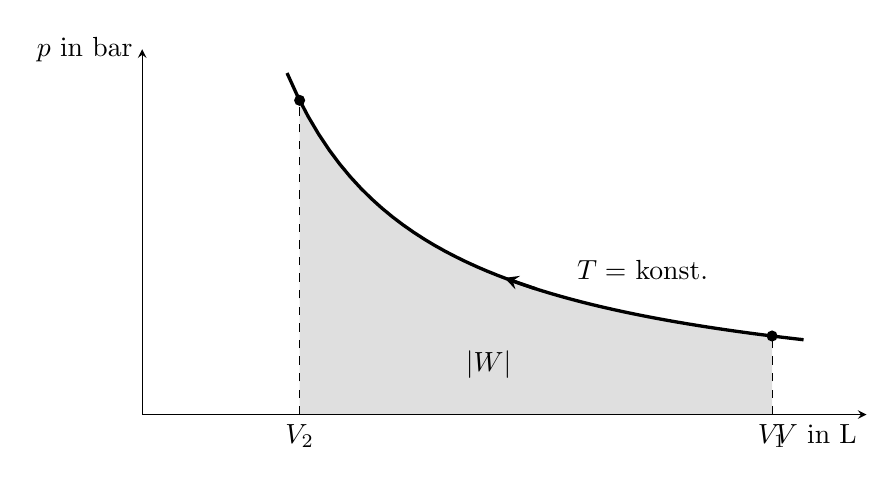
\begin{tikzpicture}[>=stealth, x=0.4cm, y=0.8cm]
 \fill[gray!25] (5,0) -- plot[domain=5:20, samples=40] (\x,{24.94/\x}) -- (20,0) -- cycle;
 \draw[->] (0,0) -- (23,0) node[below left] {$V$ in L};
 \draw[->] (0,0) -- (0,5.8) node[left] {$p$ in bar};
 \draw[very thick] plot[domain=4.6:21, samples=50] (\x,{24.94/\x});
 \draw[->, very thick] (12.5,{24.94/12.5}) -- (11.5,{24.94/11.5});
 \draw[dashed] (5,0) node[below] {$V_2$} -- (5,4.988);
 \draw[dashed] (20,0) node[below] {$V_1$} -- (20,1.247);
 \fill (5,4.988) circle (2pt) (20,1.247) circle (2pt);
 \node at (11,0.8) {$|W|$};
 \node[anchor=west] at (13.5,2.3) {$T = $ konst.};
\end{tikzpicture}
\end{center}

Bei konstanter Temperatur ist $p = nRT/V$. Die Arbeit, die beim Zusammendrücken am Gas verrichtet werden muss, ist die Fläche unter der Isotherme:
\begin{align}
 W &= -\int_{V_1}^{V_2} p\,\mathrm{d}V = -nRT\int_{V_1}^{V_2}\frac{\mathrm{d}V}{V} = nRT\,\ln\frac{V_1}{V_2}
\end{align}
Mit den gegebenen Werten:
\begin{align}
 W &= \WisoF \\
   &= \nLu\cdot\ncR\cdot\TL\cdot\ln\frac{\VaO}{\VbO} \\
   &= \Wiso \approx \result{\WisoP{3}{2}}
\end{align}
Die innere Energie bleibt dabei gleich: Diese Energie gibt die Luft als Wärme an die Umgebung ab.
